\documentclass[conference,a4paper]{IEEEtran}
\usepackage{cite}
\usepackage{amsmath,amssymb}
\usepackage{graphicx,booktabs}
\usepackage{algorithm,algpseudocode}
\usepackage[hidelinks,pdfauthor={}]{hyperref}
\hypersetup{pdftitle={Evaluating Instance Filtering and Attribute Weighting in Decision Tree--Naive Bayes Hybrids},pdfauthor={},pdfsubject={Empirical evaluation of supervised cleaning},pdfkeywords={Naive Bayes, decision tree, instance filtering, attribute weighting, cross-validation}}
\begin{document}
\title{Evaluating Instance Filtering and Attribute Weighting in Decision Tree--Naive Bayes Hybrids}
\author{}
\maketitle

\begin{abstract}
We evaluate two published cleaning steps for decision tree and Naive Bayes (NB) classifiers: an NB judge removes training rows that it misclassifies, and a tree selects and weights attributes for NB. We compare each step alone, both sequential orders, and a parallel design that derives rows and attributes independently. Twelve settings are evaluated on ten public datasets using ten repetitions of stratified 10-fold cross-validation. Every supervised step is fitted within the training fold, and every held-out row is scored. Plain C4.5 averages 86.33\% accuracy, compared with 81.21\% and 80.89\% for the two sequential tree methods. Attribute weighting alone gives the highest mean NB accuracy, 77.35\%, compared with 75.93\% for plain NB and 75.63\% and 76.35\% for the sequential methods. None of eight exploratory paired accuracy tests is significant after Holm adjustment. Cleaning before cross-validation raises filter-based scores by 13.50--16.51 percentage points, but changes both label access and the evaluated population. Class-specific records show unequal deletion. The results do not establish a benefit from combining these steps. They support evaluating supervised cleaning within folds and reporting which classes lose training rows.
\end{abstract}
\begin{IEEEkeywords}
Naive Bayes, decision tree, instance filtering, attribute weighting, cross-validation
\end{IEEEkeywords}

\section{Introduction}
Training data can be changed before a classifier is fitted. An instance filter decides which rows remain, while attribute selection decides which columns remain. Farid et al.~\cite{farid2014hybrid} proposed two decision tree--Naive Bayes hybrids using these operations. Algorithm 1 fits Naive Bayes (NB), deletes training rows whose predictions disagree with their supplied labels, and fits a decision tree. Algorithm 2 fits a tree, keeps the attributes that it tests, and uses their tree depths to weight NB likelihoods. We study whether applying these two steps together helps, and whether their order matters.

The steps can affect each other. Removing rows first changes the examples available to the attribute-selection tree. Selecting attributes first changes the inputs to the filtering model, which we call the judge. When its likelihoods also receive the tree weights, the judge can reject a different set of rows. A combined method therefore needs to be compared with the individual steps and the uncleaned classifier.

Evaluation placement also matters. A filter fitted before cross-validation (CV) can use labels of future test cases and remove some of those cases from evaluation. A filter fitted inside a training fold has no such access, and the test fold retains all its rows. These procedures answer different questions. Their score difference cannot by itself separate information leakage from the change in the population being scored.

We ask whether combining the steps improves predictive performance, whether their order and independent composition change the results, and how evaluation placement and class-specific deletion affect interpretation. We compare twelve arms on ten datasets using shared splits and fixed learner settings.

\section{Related Work}
Farid et al.~\cite{farid2014hybrid} provide the two hybrids that motivate our study. Hall~\cite{hall2007decision} studied tree-based attribute weighting for NB. We use a single pruned C4.5 tree to derive weights. Our comparison adds both sequential orders and an independent parallel reference, with either NB or C4.5 as the final classifier.

Disagreement with a fitted classifier is not a verified label error. Brodley and Friedl~\cite{brodley1999identifying} studied mislabeled-data identification with classifier-based filters. Their work motivates examining how rejection rules interact with useful training examples. Confident Learning~\cite{northcutt2021confident} estimates uncertainty in dataset labels through a different procedure. In this study, filtering means rejection by the specified NB judge, without assuming that the rejected label is wrong.

Evaluation bias from information shared across fitting and testing has been examined by Cawley and Talbot~\cite{cawley2010overfitting} and Kapoor and Narayanan~\cite{kapoor2023leakage}. Demircio\u{g}lu~\cite{demircioglu2021measuring} studied incorrect feature-selection placement during CV in radiomics. These works support separating supervised preprocessing from held-out evaluation. Our protocol comparison also changes the scored sample when rows are deleted, so it is a descriptive sensitivity analysis rather than an isolated estimate of leakage bias. For inference across classifiers, we follow the dataset-level comparison perspective of Dem\v{s}ar~\cite{demsar2006statistical}, with the limits of a ten-dataset benchmark stated explicitly.

\section{Methods}
\subsection{Algorithm 1: Instance Filtering}
Let $D$ denote the current training rows and their supplied labels. We fit an NB judge on $D$ and predict those same rows. A row remains when the predicted label equals its supplied label. The final classifier is then fitted again on the retained data. Algorithm 1 ends in C4.5; we also use the same filtering step followed by NB as a reference arm. The judge's predictions are in-sample decisions, not out-of-fold estimates of label quality.

A safeguard retains the original training rows if deletion would leave fewer than two classes. This prevents a one-class training set but does not preserve every class in a multiclass dataset. The safeguard was not triggered in the stored runs. Even without triggering it, a judge can remove every training example of one rare class. We therefore record removal rates by class rather than relying only on total deletion.

\subsection{Algorithm 2: Attribute Selection and Weighting}
We fit a C4.5 tree on the current training data. Let $d_j$ be the smallest depth at which the tree tests attribute $j$, with its root at depth one. Let $S$ be the set of tested attributes. We assign the weight
\begin{equation}
w_j=\begin{cases}1/\sqrt{d_j},&j\in S,\\0,&j\notin S.\end{cases}
\label{eq:weights}
\end{equation}
Untested attributes are dropped. Attributes used closer to the root have larger weights. For a class $c$ and input $x$, NB uses the log score
\begin{equation}
s_c(x)=\log P(c)+\sum_{j\in S}w_j\log P(x_j\mid c).
\label{eq:nb}
\end{equation}
Here $P(c)$ is the training class prior and $P(x_j\mid c)$ is the class-conditional likelihood. The predicted class has the largest score. We use add-one counts for nominal attributes and Gaussian likelihoods for numeric attributes. The weights scale likelihood terms; they do not change the supplied labels.

Algorithm 2 ends in weighted NB. Its C4.5 reference uses the selected columns, but the final tree does not use NB's likelihood weights. We use \emph{support} to mean passing Algorithm 2's weights to an NB judge or final NB. This distinguishes column selection from weighting an NB model on those columns.

\subsection{Sequential Paths and Parallel Reference}
Path 1, denoted NA, runs instance filtering first with a plain NB judge. It then derives attributes and weights from a tree fitted on the retained rows. Path 2, denoted AN, derives attributes and weights from the original training fold and then filters using weighted NB with support enabled. The same weights reach the Path 2 judge and its final NB. They are not re-estimated after deletion. Both paths end in either NB or C4.5, giving four sequential settings.

The parallel design, P, derives the retained rows and selected attributes independently from the original training fold. Its plain NB judge sees all original columns. Its selection tree sees all original training rows. We then take the retained rows restricted to the selected columns, and fit the final classifier on that intersection. The final NB receives the tree's weights. This provides a reference for combining both operations without letting either operation change the input used to fit the other.

\setcounter{algorithm}{2}
\begin{algorithm}[t]
\caption{Training a combined method on one fold}
\label{alg:paths}
\begin{algorithmic}[1]
\Require Training data $D$, design $o\in\{\mathrm{NA},\mathrm{AN},\mathrm{P}\}$, final learner $L$
\If{$o=\mathrm{NA}$}
 \State $R\gets\Call{Filter}{D,\text{plain NB}}$
 \State $(S,W)\gets\Call{Select}{D[R,:],\text{C4.5}}$
\ElsIf{$o=\mathrm{AN}$}
 \State $(S,W)\gets\Call{Select}{D,\text{C4.5}}$
 \State $R\gets\Call{Filter}{D[:,S],\text{NB with }W}$
\Else
 \State $R\gets\Call{Filter}{D,\text{plain NB}}$
 \State $(S,W)\gets\Call{Select}{D,\text{C4.5}}$
\EndIf
\State Fit $L$ on $D[R,S]$; NB uses $W$
\State \Return fitted classifier and selected columns $S$
\end{algorithmic}
\end{algorithm}

Algorithm~\ref{alg:paths} uses the filtering safeguard above. If a selection tree tests no attribute, a combined design keeps all current columns with unit weights. The standalone Algorithm 2--NB implementation instead uses zero attribute weights and predicts from the priors. No empty-selection event occurred in the stored runs. At prediction time, the held-out rows lose the same columns as the training data. They never lose rows.

\section{Experimental Method}
\subsection{Datasets and Learners}
We use the ten dataset names from the 2014 study: breast cancer, contact lenses, diabetes, glass, iris, soybean, vote, image segmentation, tic-tac-toe, and NSL-KDD. Table~\ref{tab:data} gives their row, attribute and class counts. Their sizes range from 24 rows for contact lenses to 25,192 for NSL-KDD. Image segmentation combines two UCI files into 2,310 rows, whereas the earlier study lists 1,500, and NSL-KDD uses the 20\% training file~\cite{tavallaee2009detailed}. Glass and NSL-KDD each have one fewer class in our files than the earlier study lists. These copies permit matched comparisons within this study, but do not establish an exact reproduction of the original data preparation.

\begin{table}[t]
\caption{Files used in this study. Attributes are original columns; the final column is the smallest class size.}
\label{tab:data}
\centering\footnotesize
\setlength{\tabcolsep}{4pt}
\begin{tabular}{lrrrr}
\toprule
Dataset & Rows & Attr. & Classes & Min. \\
\midrule
Breast cancer & 286 & 9 & 2 & 85 \\
Contact lenses & 24 & 4 & 3 & 4 \\
Diabetes & 768 & 8 & 2 & 268 \\
Glass & 214 & 9 & 6 & 9 \\
Segmentation & 2310 & 19 & 7 & 330 \\
Iris & 150 & 4 & 3 & 50 \\
NSL-KDD & 25192 & 41 & 22 & 1 \\
Soybean & 683 & 35 & 19 & 8 \\
Tic-tac-toe & 958 & 9 & 2 & 332 \\
Vote & 435 & 16 & 2 & 168 \\
\bottomrule
\end{tabular}

\end{table}

C4.5 is Weka~\cite{witten2016weka} J48 3.8.6 with pruning and options \texttt{-C 0.25 -M 2}. NB is the implementation named FaithfulNB, using add-one nominal counts and variance-smoothed Gaussian likelihoods. We retain original attribute columns, including nominal columns, rather than expanding them into one-hot indicators. Tree depths therefore refer to original attributes.

Nominal vocabularies are obtained from the complete files and fixed across folds. Missing nominal tokens form a separate category. Priors, nominal counts, numeric distributions, selection trees, and judges are fitted on training rows in the main protocol. Full-file vocabularies remain a limitation of the evaluation, even though supervised fitting stays within the training fold. We use fixed settings without hyperparameter search or nested tuning.

\subsection{Protocols and Arms}
Protocol B is the main evaluation. We use stratified 10-fold CV with seeds 0--9, producing 100 folds per dataset and method. Every arm shares the same split for a given dataset and seed. The judge, selection tree, and final classifier are fitted within the training fold. Every held-out case is scored. The twelve arms are the two plain classifiers and five cleaning designs, N, A, NA, AN, and P, each followed by NB or C4.5. N and A denote the individual filtering and attribute steps.

Protocol A first fits cleaning on the whole dataset, then cross-validates the final classifier on the cleaned data. Its supervised steps see future test labels, and filtering changes which rows enter CV. For filtering arms, the evaluated row pool and resulting folds can differ between protocols. Attribute-only arms retain the shared folds. We report these protocol contrasts descriptively. Protocol A is a diagnostic procedure and is not used for headline performance estimates.

\subsection{Measures and Exploratory Tests}
We report accuracy and macro-F1 as percentages. For each dataset and method, we average the 100 fold scores with equal fold weight. Benchmark summaries then give each dataset equal weight. Their spread is the standard deviation of ten seed-level benchmark averages, not a confidence interval from ten independent datasets.

Macro-F1 averages class F1 over the union of classes present in a fold's true labels and predictions, with zero for undefined F1. The class set can change between folds. This is the saved scoring convention, not a fixed-class pooled-prediction score. We retain accuracy as the endpoint for the inferential comparisons and use macro-F1 descriptively.

We retain eight two-sided Wilcoxon signed-rank accuracy tests on the ten paired dataset averages. They compare Algorithm 1--DT and Algorithm 2--NB with their respective baselines, the four sequential methods with their respective baselines, and AN with NA for each final classifier. Exact permutation enumeration is used, with Holm adjustment across all eight tests at 0.05. Zero differences are dropped, so the N--DT and NA--DT contrasts use nine datasets. This family was added during revision after observing the saved results, so the tests are exploratory. Parallel and single-step-versus-combined comparisons are descriptive additions, not extra tests selected for significance. Nonsignificance does not establish equivalence. All differences below are in percentage points (pp).

\section{Results}
\subsection{Predictive Performance}
Table~\ref{tab:summary} reports all twelve Protocol B settings. Plain C4.5 has the highest benchmark means, 86.33\% accuracy and 81.92\% macro-F1. NA--DT reaches 81.21\% accuracy and AN--DT reaches 80.89\%, giving descriptive losses of 5.12 and 5.44 pp. Their macro-F1 means are also lower, 75.76\% and 73.93\%. Filtering alone reaches 81.03\% accuracy, so adding selection after filtering recovers 0.18 pp on average under these settings.

\begin{table}[t]
\caption{Protocol B scores (\%). Means give datasets equal weight; SD describes ten seed-level benchmark averages. F1 denotes macro-F1. Base is uncleaned; N, A, NA, AN, and P are defined in the text.}
\label{tab:summary}
\centering\footnotesize
\setlength{\tabcolsep}{3pt}
\begin{tabular}{lrrrr}
\toprule
Arm & Acc. & SD & F1 & SD \\
\midrule
Base--NB & 75.93 & 0.32 & 69.80 & 0.52 \\
N--NB & 75.42 & 0.46 & 69.08 & 0.46 \\
A--NB & 77.35 & 0.41 & 71.73 & 0.63 \\
NA--NB & 75.63 & 0.45 & 69.60 & 0.72 \\
AN--NB & 76.35 & 0.34 & 69.91 & 0.60 \\
P--NB & 76.39 & 0.37 & 70.47 & 0.68 \\
Base--DT & 86.33 & 0.33 & 81.92 & 0.44 \\
N--DT & 81.03 & 0.37 & 75.70 & 0.63 \\
A--DT & 86.19 & 0.33 & 81.84 & 0.42 \\
NA--DT & 81.21 & 0.29 & 75.76 & 0.58 \\
AN--DT & 80.89 & 0.45 & 73.93 & 0.80 \\
P--DT & 81.05 & 0.34 & 75.58 & 0.58 \\
\bottomrule
\end{tabular}

\end{table}

For NB, attribute weighting alone gives the highest mean accuracy, 77.35\%, compared with 75.93\% for plain NB. NA--NB and AN--NB reach 75.63\% and 76.35\%. Their changes from plain NB are $-0.30$ and $+0.42$ pp, and both trail attribute weighting alone. Selecting attributes before C4.5 leaves its mean almost unchanged at 86.19\%.

\begin{table*}[t]
\caption{Protocol B accuracy by dataset (\%). NB and DT panels use the same six designs. P derives retained rows and selected columns independently from the original training fold.}
\label{tab:datasets}
\centering\footnotesize
\setlength{\tabcolsep}{4pt}
\begin{tabular}{lrrrrrrrrrrrr}
\toprule
 & \multicolumn{6}{c}{Final NB} & \multicolumn{6}{c}{Final DT (J48)} \\
\cmidrule(lr){2-7}\cmidrule(lr){8-13}
Dataset & Base & N & A & NA & AN & P & Base & N & A & NA & AN & P \\
\midrule
Breast cancer & 72.12 & 72.68 & 72.43 & 71.28 & 72.53 & 72.46 & 74.84 & 71.77 & 73.91 & 71.77 & 72.08 & 71.20 \\
Contact lenses & 73.00 & 73.00 & 80.67 & 83.00 & 79.33 & 83.00 & 84.67 & 84.67 & 84.67 & 84.67 & 80.67 & 84.67 \\
Diabetes & 75.52 & 74.41 & 76.73 & 75.58 & 75.67 & 75.81 & 74.12 & 75.12 & 74.18 & 75.23 & 75.57 & 74.86 \\
Glass & 45.95 & 37.00 & 47.84 & 30.93 & 37.28 & 32.29 & 66.58 & 48.83 & 66.58 & 48.97 & 49.15 & 48.65 \\
Segmentation & 79.76 & 74.92 & 82.30 & 74.53 & 77.32 & 76.57 & 96.81 & 89.24 & 96.83 & 89.26 & 90.88 & 89.79 \\
Iris & 95.53 & 95.33 & 95.40 & 95.33 & 95.87 & 95.60 & 94.27 & 94.93 & 94.27 & 94.93 & 93.80 & 94.93 \\
NSL-KDD & 67.42 & 75.79 & 62.80 & 74.53 & 75.23 & 76.16 & 99.47 & 87.43 & 99.47 & 89.68 & 87.07 & 88.37 \\
Soybean & 90.09 & 89.00 & 89.40 & 85.67 & 86.66 & 86.95 & 92.71 & 88.71 & 92.26 & 87.89 & 90.98 & 88.24 \\
Tic-tac-toe & 69.83 & 71.89 & 70.68 & 70.03 & 68.07 & 69.72 & 84.74 & 74.43 & 84.74 & 74.55 & 73.17 & 74.43 \\
Vote & 90.06 & 90.13 & 95.24 & 95.45 & 95.49 & 95.36 & 95.08 & 95.13 & 95.03 & 95.13 & 95.54 & 95.38 \\
\bottomrule
\end{tabular}

\end{table*}

The per-dataset results in Table~\ref{tab:datasets} show variation hidden by the means. On glass, NA--NB falls from the plain NB baseline of 45.95\% to 30.93\%; NA--DT falls from 66.58\% to 48.97\%. On contact lenses, NA--NB increases from 73.00\% to 83.00\%. That result comes from only 24 rows, reused by every repeated split, and has limited evidence for generalization. The dataset still receives the same benchmark weight as the other nine datasets.

\begin{figure}[t]
\centering
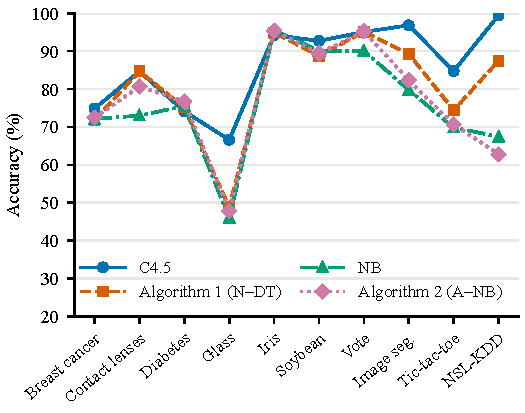
\includegraphics[width=\columnwidth]{figures/single_steps.pdf}
\caption{Protocol B accuracy of the base classifiers and the two published hybrids on each dataset, in the dataset order of the 2014 study. Lines join datasets only for readability.}
\label{fig:single}
\end{figure}

Figure~\ref{fig:single} draws the per-dataset comparison in the style and dataset order of the 2014 study. In the 2014 tables, Algorithm 1 exceeds C4.5 and Algorithm 2 exceeds NB on all ten datasets. Under Protocol B, Algorithm 1 lies below C4.5 on six datasets, by up to 17.75 pp on glass, matches it on contact lenses, and is higher only on diabetes, iris and vote, by less than 1 pp. Algorithm 2 lies above NB on seven datasets, most clearly on contact lenses (+7.67 pp) and vote (+5.18 pp). It falls below NB on iris, soybean and NSL-KDD, where it loses 4.62 pp.

\begin{figure}[t]
\centering
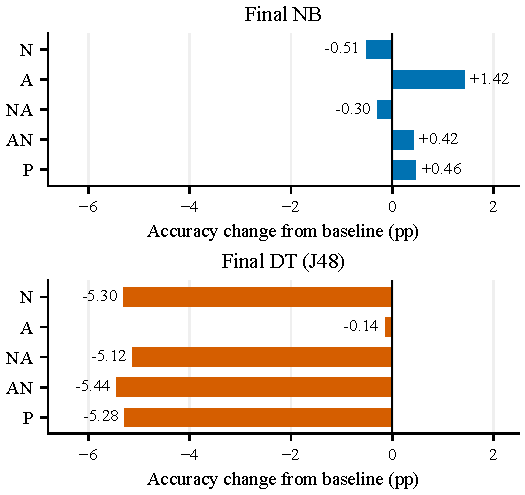
\includegraphics[width=\columnwidth]{figures/accuracy_change.pdf}
\caption{Protocol B mean accuracy change from the corresponding uncleaned classifier. Each dataset receives equal weight. Bars describe numerical changes and do not indicate statistical significance.}
\label{fig:accuracy}
\end{figure}

\subsection{Order and Independent Composition}
Figure~\ref{fig:accuracy} shows the mean baseline differences. Table~\ref{tab:tests} gives the retained paired tests. AN--DT has a raw $p=0.014$ against plain C4.5, but its Holm-adjusted $p=0.109$ exceeds 0.05. None of the eight comparisons is significant after adjustment.

\begin{table}[t]
\caption{Exploratory paired dataset-level accuracy tests. Differences are first method minus second. Holm adjustment covers the eight displayed tests.}
\label{tab:tests}
\centering\footnotesize
\setlength{\tabcolsep}{3pt}
\begin{tabular}{lrrr}
\toprule
Contrast & $\Delta$ & $p$ & Holm $p$ \\
\midrule
N--DT vs. DT & -5.30 & 0.055 & 0.383 \\
A--NB vs. NB & +1.42 & 0.131 & 0.654 \\
NA--DT vs. DT & -5.12 & 0.055 & 0.383 \\
AN--DT vs. DT & -5.44 & 0.014 & 0.109 \\
NA--NB vs. NB & -0.30 & 1.000 & 1.000 \\
AN--NB vs. NB & +0.42 & 0.846 & 1.000 \\
AN--DT vs. NA--DT & -0.32 & 0.922 & 1.000 \\
AN--NB vs. NA--NB & +0.71 & 0.275 & 1.000 \\
\bottomrule
\end{tabular}

\end{table}

Moving from NA to AN raises NB mean accuracy by 0.71 pp and lowers C4.5 mean accuracy by 0.32 pp. Raw $p$ values are 0.275 and 0.922. We find no statistically established order advantage under these settings. This comparison includes a change from a plain to a supported judge, so it does not isolate ordering while keeping judge inputs and weights fixed.

The parallel reference reaches 76.39\% accuracy with NB and 81.05\% with C4.5. NA differs from P by $-0.76$ pp for NB and $+0.16$ pp for C4.5. AN differs from P by $-0.05$ and $-0.16$ pp, respectively. These descriptive differences do not show a consistent benefit from chaining.

\begin{figure}[t]
\centering
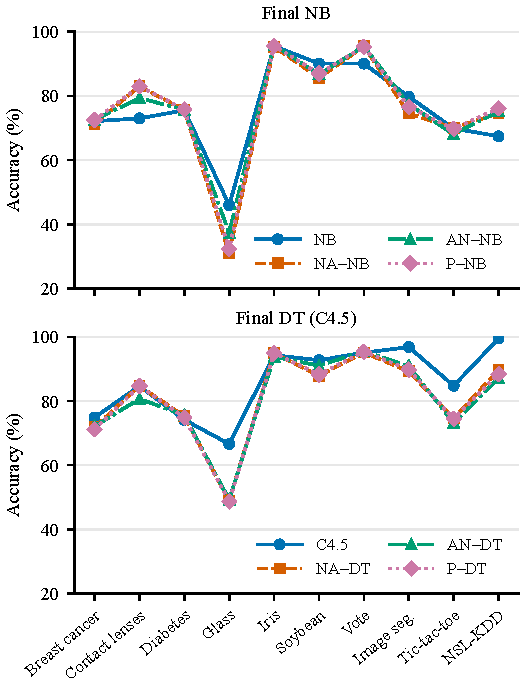
\includegraphics[width=\columnwidth]{figures/combined_paths.pdf}
\caption{Protocol B accuracy of the three combined designs and the uncleaned classifier on each dataset, with final NB (top) and final C4.5 (bottom). Lines join datasets only for readability.}
\label{fig:combined}
\end{figure}

Figure~\ref{fig:combined} shows the combined designs dataset by dataset. With final C4.5, the three lines nearly coincide and stay below the plain tree on glass, image segmentation, tic-tac-toe and NSL-KDD, by 5.93 to 17.94 pp. On those four datasets, the designs differ from one another by at most 2.60 pp. With final NB, the combined designs gain 6.33 to 10.00 pp on contact lenses, 5.29 to 5.43 pp on vote and 7.11 to 8.75 pp on NSL-KDD, but lose 8.68 to 15.03 pp on glass. The dataset changes the outcome far more than the choice among NA, AN and P.

\subsection{Cleaning Before Cross-Validation}
Table~\ref{tab:protocols} contrasts the two protocols. N--DT reaches 94.52\% after full-data filtering, compared with 81.03\% under within-fold fitting, a difference of 13.50 pp calculated from unrounded means. NA--DT and AN--DT rise to 94.72\% and 96.32\%. Across filter-based settings, differences range from 13.50 to 16.51 pp. Attribute-only differences are smaller, 0.72 pp for NB and 0.33 pp for C4.5.

\begin{table}[t]
\caption{Mean accuracy (\%) under within-fold cleaning (B) and cleaning before CV (A). A changes label access and, for filtering arms, the evaluated population. Differences use unrounded means.}
\label{tab:protocols}
\centering\footnotesize
\setlength{\tabcolsep}{3pt}
\begin{tabular}{lrrr}
\toprule
Arm & A (\%) & B (\%) & A$-$B (pp) \\
\midrule
N--NB & 91.93 & 75.42 & +16.51 \\
A--NB & 78.07 & 77.35 & +0.72 \\
NA--NB & 90.11 & 75.63 & +14.48 \\
AN--NB & 91.08 & 76.35 & +14.74 \\
P--NB & 91.10 & 76.39 & +14.71 \\
N--DT & 94.52 & 81.03 & +13.50 \\
A--DT & 86.52 & 86.19 & +0.33 \\
NA--DT & 94.72 & 81.21 & +13.51 \\
AN--DT & 96.32 & 80.89 & +15.43 \\
P--DT & 94.67 & 81.05 & +13.62 \\
\bottomrule
\end{tabular}

\end{table}

Protocol B asks the classifier to predict all held-out rows. Protocol A uses a supervised judge to choose which rows can enter the subsequent evaluation. Removing difficult cases may contribute to the higher scores, but the experiment does not identify its separate contribution. For filtering arms, the labels available during cleaning, the sample, and the resulting folds change together. Attribute-only cleaning retains every row but still uses future test information for selection. Its smaller score change does not justify selecting attributes before CV.

\subsection{Class Representation After Filtering}
Figure~\ref{fig:removal} shows class-specific deletion for breast cancer. The plain judge removes an average of 50.63\% of recurrence-event training rows and 14.51\% of no-recurrence-event rows. After attribute selection, the supported judge removes 58.97\% and 11.72\%, respectively. Each rate uses that class's training-row count as its denominator, not the size of the entire dataset.

\begin{figure}[t]
\centering
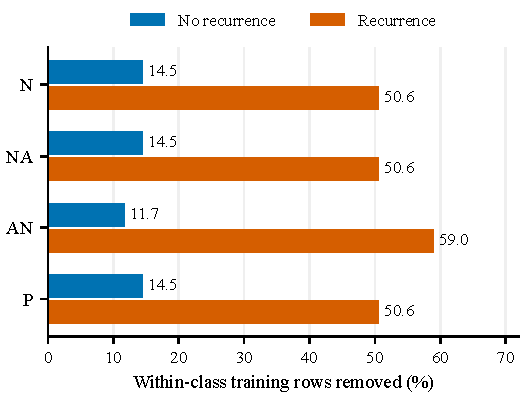
\includegraphics[width=\columnwidth]{figures/class_removal.pdf}
\caption{Breast-cancer training-row deletion by class, averaged over Protocol B folds. N, NA and P share the plain-judge mask; AN uses a supported judge after A. Rates describe rejection, not verified label errors.}
\label{fig:removal}
\end{figure}

The minority class loses a larger fraction of its examples in both cases. The records cannot establish whether the rejected labels were wrong or the judge failed on valid cases. Selection also changes after deletion. On glass, the tree retains 97.00\% of attributes on the original training fold and 61.00\% after plain filtering. On vote, retention falls from 27.38\% to 7.62\%. The operations interact in their fitted outputs even though we have not established a predictive advantage for one order.

\section{Discussion and Limitations}
Under the tested settings, combining filtering and weighting does not establish a predictive advantage. Neither sequential NB mean exceeds attribute weighting alone. Lower tree means and unequal class deletion indicate that retained class composition matters. We have no verified natural label-error annotations or matched comparison with modern label-cleaning methods.

Our benchmark uses an older dataset family with file and class-count differences from the 2014 tables. The NSL-KDD C4.5 baseline remains an unresolved discrepancy: 99.47\% here versus 71.11\% previously reported. Over the ten datasets, the 2014 tables average 88.43\% for Algorithm 1 and 83.42\% for Algorithm 2, against 83.52\% for C4.5 and 77.33\% for NB. Under Protocol B, Algorithm 1 is 5.30 pp below C4.5 rather than above it, and Algorithm 2 exceeds NB by 1.42 pp rather than 6.09 pp. Figure~\ref{fig:reported} shows the per-dataset values. The reported Algorithm 1 accuracy lies between our two protocols on seven datasets, and the reported Algorithm 2 accuracy exceeds both on eight. File differences prevent attributing these gaps to a single cause, so this is not an exact replication. The evidence concerns our shared files, implementation, and splits.

\begin{figure}[t]
\centering
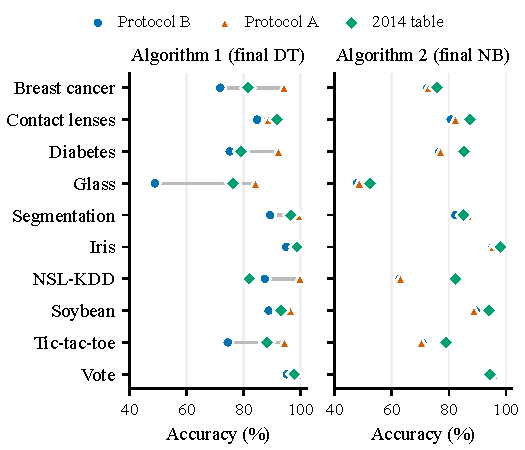
\includegraphics[width=\columnwidth]{figures/reported_protocols.pdf}
\caption{Accuracy of Algorithm 1 (top) and Algorithm 2 (bottom) on each dataset under Protocols B and A, beside the 2014 table values for each algorithm and its base classifier. Glass, image segmentation and NSL-KDD files differ from the 2014 study, so the comparison is descriptive.}
\label{fig:reported}
\end{figure}

Rare classes limit interpretation. Contact lenses contains classes with four and five rows. NSL-KDD has classes with fewer than ten examples, including a singleton. Some stratified folds consequently lack a class in training or testing. Repeating splits does not create new examples, and macro-F1 may average different class sets across folds. These results cannot establish reliable rare-class performance.

Full-file nominal vocabularies leave deployment with unseen categories untested. Ten datasets limit inference after multiplicity adjustment; more split seeds would not add independent datasets. The A/B contrast cannot establish the original study's evaluation procedure or isolate a causal leakage effect.

A useful next study would hold the scored population fixed while varying access during cleaning. A separate matched judge ablation could distinguish ordering from support. For the present methods, we recommend fitting supervised cleaning within each training fold, scoring every held-out row, and reporting class-specific removal alongside predictive metrics.

\section{Conclusion}
We compared instance filtering and tree-based attribute weighting alone, in both sequential orders, and in an independent parallel design. On ten datasets with shared within-fold evaluation, combined tree methods have lower mean accuracy than plain C4.5, and combined NB methods trail attribute weighting alone. Eight exploratory paired accuracy tests establish no significant difference after Holm adjustment. Higher before-CV scores involve a changed evaluation population as well as different information access. The removal records show unequal class loss. For these settings, the comparison supports keeping cleaning inside training folds and reporting the class composition of the retained data.

\section*{Acknowledgment}
Large language models assisted with drafting, language revision, typesetting, and preparation of figures and tables from saved results. The authors are responsible for the manuscript content and accuracy.

\bibliographystyle{IEEEtran}
\bibliography{references}
\end{document}
